% Options for packages loaded elsewhere
\PassOptionsToPackage{unicode}{hyperref}
\PassOptionsToPackage{hyphens}{url}
%
\documentclass[
]{article}
\usepackage{amsmath,amssymb}
\usepackage{lmodern}
\usepackage{iftex}
\ifPDFTeX
  \usepackage[T1]{fontenc}
  \usepackage[utf8]{inputenc}
  \usepackage{textcomp} % provide euro and other symbols
\else % if luatex or xetex
  \usepackage{unicode-math}
  \defaultfontfeatures{Scale=MatchLowercase}
  \defaultfontfeatures[\rmfamily]{Ligatures=TeX,Scale=1}
\fi
% Use upquote if available, for straight quotes in verbatim environments
\IfFileExists{upquote.sty}{\usepackage{upquote}}{}
\IfFileExists{microtype.sty}{% use microtype if available
  \usepackage[]{microtype}
  \UseMicrotypeSet[protrusion]{basicmath} % disable protrusion for tt fonts
}{}
\makeatletter
\@ifundefined{KOMAClassName}{% if non-KOMA class
  \IfFileExists{parskip.sty}{%
    \usepackage{parskip}
  }{% else
    \setlength{\parindent}{0pt}
    \setlength{\parskip}{6pt plus 2pt minus 1pt}}
}{% if KOMA class
  \KOMAoptions{parskip=half}}
\makeatother
\usepackage{xcolor}
\usepackage[margin=1in]{geometry}
\usepackage{longtable,booktabs,array}
\usepackage{calc} % for calculating minipage widths
% Correct order of tables after \paragraph or \subparagraph
\usepackage{etoolbox}
\makeatletter
\patchcmd\longtable{\par}{\if@noskipsec\mbox{}\fi\par}{}{}
\makeatother
% Allow footnotes in longtable head/foot
\IfFileExists{footnotehyper.sty}{\usepackage{footnotehyper}}{\usepackage{footnote}}
\makesavenoteenv{longtable}
\usepackage{graphicx}
\makeatletter
\def\maxwidth{\ifdim\Gin@nat@width>\linewidth\linewidth\else\Gin@nat@width\fi}
\def\maxheight{\ifdim\Gin@nat@height>\textheight\textheight\else\Gin@nat@height\fi}
\makeatother
% Scale images if necessary, so that they will not overflow the page
% margins by default, and it is still possible to overwrite the defaults
% using explicit options in \includegraphics[width, height, ...]{}
\setkeys{Gin}{width=\maxwidth,height=\maxheight,keepaspectratio}
% Set default figure placement to htbp
\makeatletter
\def\fps@figure{htbp}
\makeatother
\setlength{\emergencystretch}{3em} % prevent overfull lines
\providecommand{\tightlist}{%
  \setlength{\itemsep}{0pt}\setlength{\parskip}{0pt}}
\setcounter{secnumdepth}{5}
\ifLuaTeX
  \usepackage{selnolig}  % disable illegal ligatures
\fi
\IfFileExists{bookmark.sty}{\usepackage{bookmark}}{\usepackage{hyperref}}
\IfFileExists{xurl.sty}{\usepackage{xurl}}{} % add URL line breaks if available
\urlstyle{same} % disable monospaced font for URLs
\hypersetup{
  pdftitle={Customer Ratings Analysis},
  pdfauthor={Nicole Chua},
  hidelinks,
  pdfcreator={LaTeX via pandoc}}

\title{Customer Ratings Analysis}
\author{Nicole Chua}
\date{1/31/2022}

\begin{document}
\maketitle

\section{Introduction}

Our primary objective is to compare and rank the four types of
businesses (BBQ, Burgers, Pizza, Sandwiches) from unpaid customer
ratings. A customer provides ratings from 1-5 for every type of business
and each set of business ratings by a customer is designated an elite or
non-elite status. It is also possible that a customer contributes
ratings as both an elite and non-elite. We are also interested in
whether elite customers give higher ratings than non-elite customers.

Using the tall/long version of data, there are 3 non-numeric fields, 1
numeric field and 262 observations.

\section{Methods}

Since each customer rates all food types but only some are designated
both elite statuses, food types is a within factor and elite status is a
between factor. Thus, we use a repeated measures one-way ANOVA to
compare the means of ratings by food types and a separate one-way ANOVA
for elite status to test the two following sets of hypotheses:

Hypotheses for the effect of food type:

\emph{H\textsubscript{0}}: There is no difference in mean customer
rating for any food type.

\emph{H\textsubscript{a}}: There is a difference in mean customer rating
by food type.

Hypotheses for the effect of elite status:

\emph{H\textsubscript{0}}: There is no difference in mean customer
rating for any elite status.

\emph{H\textsubscript{a}}: There is a difference in mean customer rating
by elite status.

\section{Results}

\subsection{Summary statistics}

We start by computing the mean customer ratings of the four food types
split by elite vs non-elite status and for each elite status as well in
Table 1. \newpage

\begin{longtable}[]{@{}lrr@{}}
\toprule()
& FALSE & TRUE \\
\midrule()
\endhead
BBQ & 3.065000 & 3.371719 \\
Burgers & 3.749702 & 3.841094 \\
Pizza & 3.211567 & 3.747109 \\
Sandwiches & 3.966045 & 4.001953 \\
Elite & 3.498078 & 3.740469 \\
\bottomrule()
\end{longtable}

\begin{center}  
Table 1: Mean customer ratings by food types and elite status  
\end{center}

On average, the customers rated the food types in the order of
Sandwiches being the highest, followed by Burgers, Pizza and then BBQ
with the lowest average rating. Elite customers have a higher average
rating than non-elite customers by 0.242 points.

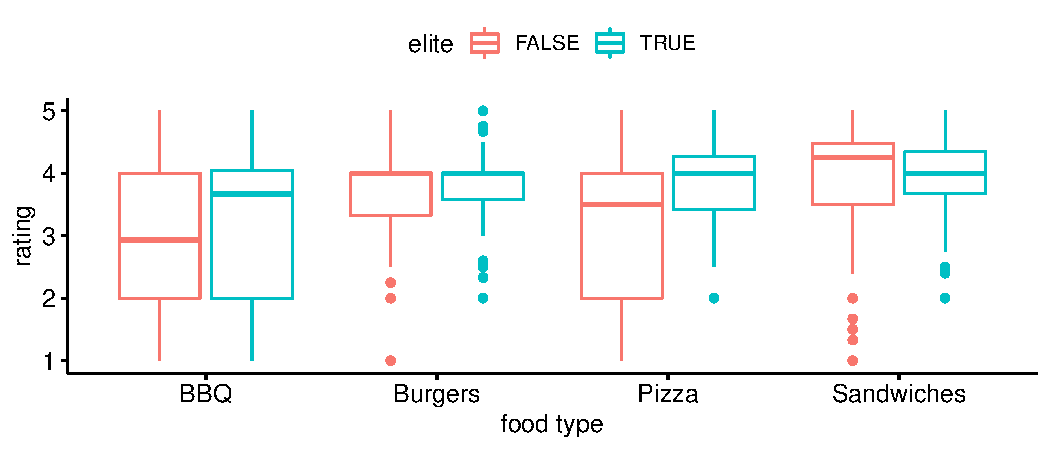
\includegraphics{customer_ratings_analysis_files/figure-latex/unnamed-chunk-3-1.pdf}

\begin{center}  
Figure 1: Box plot of mean customer ratings by food type and elite status
\end{center}

Figure 1 shows the distribution of customer ratings for each population
of food types separated by elite status.

\subsection{ANOVA models}

\begin{longtable}[]{@{}lrrrrlr@{}}
\toprule()
Effect & DFn & DFd & F & p & p\textless.05 & ges \\
\midrule()
\endhead
food\_type & 3 & 877 & 37.839 & 0 & * & 0.115 \\
\bottomrule()
\end{longtable}

\begin{center}  
Table 2: Repeated measures one-way ANOVA for food type factor  
\end{center}

\begin{longtable}[]{@{}lrrrrr@{}}
\toprule()
& Df & Sum Sq & Mean Sq & F value & Pr(\textgreater F) \\
\midrule()
\endhead
elite & 1 & 15.38524 & 15.3852398 & 16.86 & 4.34e-05 \\
Residuals & 1046 & 954.50521 & 0.9125289 & NA & NA \\
\bottomrule()
\end{longtable}

\begin{center}  
Table 3: One-way ANOVA for elite status factor  
\end{center}

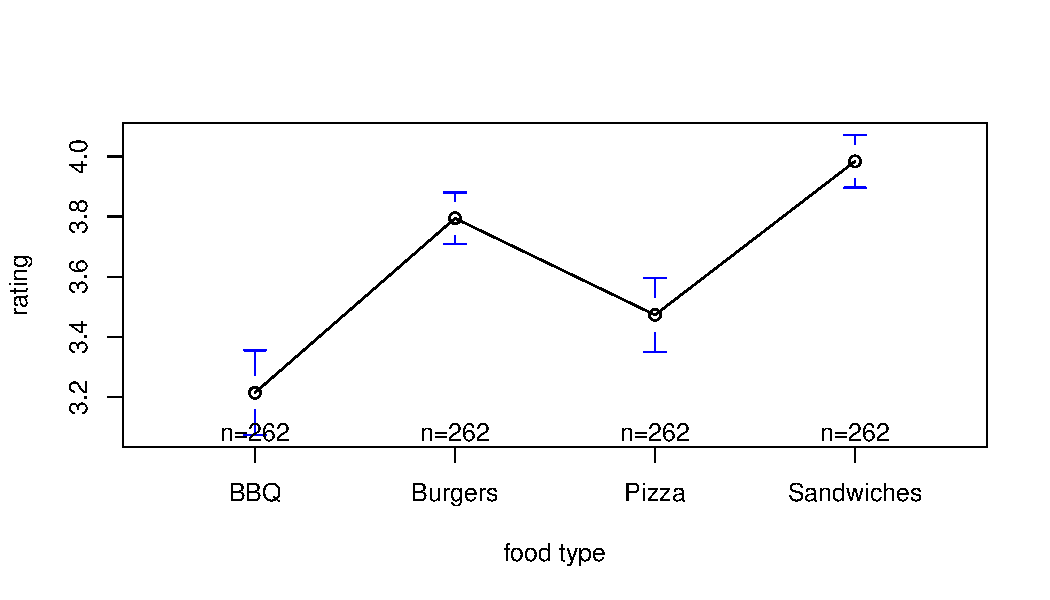
\includegraphics{customer_ratings_analysis_files/figure-latex/unnamed-chunk-5-1.pdf}

\begin{center}  
Figure 2: Plot of means and confidence intervals for food type ratings  
\end{center}

Table 2 shows the results of the repeated measures one-way ANOVA for
food types. Differences among customer ratings for different food types
are statistically significant (as indicated by the *) thus we reject the
null hypothesis and conduct Bonferroni correction post-hocs for paired
data. The results for pairwise comparisons of food types using paired t
tests and Bonferroni correction is statistically significant for all
comparisons.

Table 3 shows the results of the one-way ANOVA for elite or non-elite
status. Differences among average elite and non-elite customer ratings
are significant so we reject the null hypothesis.

Figure 2 shows the mean customer rating for each food type. Sandwiches
rank highest, followed by Burgers, Pizza and lastly, BBQ.

\section{Conclusion}

The ranking of food types according to average customer ratings are as
follows:

(highest)Sandwiches \textgreater{} Burgers \textgreater{} Pizza
\textgreater{} BBQ(lowest)

From the repeated measures one-way ANOVA test as seen in Table 2 and
Bonferroni correction test results, these differences in mean customer
ratings for food types are statistically significant for all
comparisons.

As for elite and non-elite customers, yes a customer with Elite = TRUE
gives, on average, a higher rating than a customer with Elite = FALSE.
From the one-way ANOVA for elite and non-elite status conducted in Table
3, elite customer ratings are 0.242 points higher than non-elite
customer ratings and this difference is statistically significant.

\end{document}
